Tools are necessary to test concurrency, the standard approach does
not suffice.  In this chapter we present and evaluate \dejafu{}, our
library for testing concurrency in Haskell.  We discuss the scope of
the tool~\sref{dejafu-scope} and present our abstraction over the GHC
Haskell concurrency functionality~\sref{dejafu-monadconc}.  We then
show an example of a small logic puzzle which we can represent as a
concurrent program~\sref{dejafu-100}.  We explain how programs using
our abstraction are executed~\sref{dejafu-execution} and
tested~\sref{dejafu-testing}, and argue the correctness of the testing
approach~\sref{dejafu-correctness}.  We present three case
studies~\sref{dejafu-casestudies}, evaluate the usefulness of
\dejafu{} for testing pre-existing code~\sref{dejafu-evaluation}, and
finally draw conclusions and present further
work~\sref{dejafu-conclusions}.

This chapter is derived from our previous work \cite{walker2015} and
\cite{YCS-2016-503}.

\section{Scope}
\label{sec:dejafu-scope}

We aim to support most of the functionality of GHC’s concurrency API, as made
available through the Control.Concurrent and Control.Exception module
hierarchies, which does not unavoidably require support from the runtime system.

In particular, we do not support:

\begin{itemize}
\item Blocking a thread until a file descriptor becomes available, as this
  introduces an additional source of nondeterminism.
\item Throwing an exception to a thread if it becomes deadlocked, as we cannot
  reliably detect deadlock involving only a subset of threads without support
  from the garbage collector.
\item Querying which capability (OS thread) a Haskell thread is running on, as
  this introduces an additional source of nondeterminism.
\end{itemize}

We also do not yet support \emph{bound threads}: a Haskell thread which will
always run on the same, unique, OS thread.  Bound threads are essential for
using the FFI to call libraries which use thread-local state, to ensure the
Haskell thread always sees its state and never the state of another thread.  We
have a prototype implementation, which is not yet present in a released version
of \dejafu{}\footnote{\url{https://github.com/barrucadu/dejafu/issues/126}}.

\section{Abstracting over \texttt{IO}}
\label{sec:dejafu-monadconc}

Recall from \secref{sct-fundamentals} that there are three ways of implementing
a concurrency testing tool:

\begin{itemize}
\item Override the concurrency primitives of the programming language.
\item Instrument the source program.
\item Instrument the compiled program.
\end{itemize}

We adopt the first approach in \dejafu{}.  Haskell's typeclass machinery lets us
specify an interface for concurrency, and to provide different concrete
implementations.  There is one implementation using the \verb|IO| type and the
standard functions; there is another using our own type, based on continuations
which we can inspect.

\begin{listing}
  \begin{minted}{haskell}
class (Monad m, {- other constraints omitted -}) => MonadConc m where
  type MVar m :: * -> *
  -- other types omitted

  newEmptyMVar :: m (MVar m a)
  newEmptyMVar = newEmptyMVarN ""

  newEmptyMVarN :: String -> m (MVar m a)
  newEmptyMVarN _ = newEmptyMVar

  putMVar  :: MVar m a -> a -> m ()
  readMVar :: MVar m a -> m a
  takeMVar :: MVar m a -> m a
  -- other operations omitted
  \end{minted}
  \caption{A fragment of the \texttt{MonadConc} typeclass.}\label{lst:monadconc}
\end{listing}

We call our typeclass \verb|MonadConc| for monads which can do concurrency,
\lstref{monadconc} shows a fragment.  When defining an instance of this class,
the programmer must supply concrete types for the abstract types in the
interface.  They must also supply implementations of, at least, all undefined
operations.  Some operations have default definitions: for example, there are
two ways of constructing an empty \verb|MVar|.  One way takes a name, which is
displayed in debugging information, the other does not.  Each is defined in
terms of the other, and so the programmer must supply at least one.

\begin{listing}
  \begin{minted}{haskell}
instance Monad n => MonadConc (ConcT r n) where
  type MVar (ConcT r n) = MVar r
  -- other types omitted

  newEmptyMVarN n = toConc (ANewMVar n)

  putMVar  var a = toConc (\c -> APutMVar var a (c ()))
  readMVar var   = toConc (AReadMVar var)
  takeMVar var   = toConc (ATakeMVar var)
  -- other operations omitted
  \end{minted}
  \caption{A fragment of the \texttt{MonadConc} testing implementation.}\label{lst:mvarops}
\end{listing}

The type for our testing implementation is called \verb|ConcT r n|, which is a
monad that has access to \emph{references} of type \verb|r| in a monad of type
\verb|n|.  \lstref{mvarops} shows the implementation of \lstref{monadconc} for
this type.  Each concurrency operation is of the same form: we take the
arguments and wrap them up inside a data structure whose final argument is a
continuation, which is then converted into a \verb|ConcT| value.

A concurrent computation is just a large value, where we can inspect each
``step'' of the computation by looking at the data constructor used.
Constructors mostly correspond to operations in the \verb|MonadConc| class
(there are also a few extra).  We call these constructors \emph{primitive
  actions}.  A full listing is available in \appref{primops-conc}.

We make a few departures from the semantics of the \verb|IO| monad where
necessary:

\begin{itemize}
\item The \verb|getNumCapabilities| operation allows the programmer to query the
  number of capabilities.  During testing, we return ``2'', despite executing
  everything in the same OS thread.  This is to avoid special-case behaviour for
  one capability, which may reduce concurrency.
\item Runtime errors, such as pattern match failures, can be caught as
  exceptions inside \verb|IO|.  As there is no non-\verb|IO| way to do the same,
  \dejafu{} cannot.
\item The \verb|threadDelay| operation is required to yield the thread, but not
  necessarily to delay it.  This is because it is not clear how to incorporate
  time into the systematic concurrency testing model.
\end{itemize}

There is more to \verb|IO| than concurrency and exceptions.  \dejafu{} supports
testing computations with embedded \verb|IO| actions provided that the
programmer ensures that the \verb|IO| action is atomic; that it is deterministic
when executed with a fixed schedule; and that it does not block on the action of
another thread.  Failing to meet any of these conditions may lead to incomplete
testing.

\section{The 100 Prisoners Problem}
\label{sec:dejafu-100}

There's a popular logic puzzle which goes something like this:

\begin{displayquote}
  There are 100 prisoners in solitary cells.  There's a central living
  room with one light bulb.  No prisoner can see the light bulb from
  their own cell.  Everyday, the warden picks a prisoner equally at
  random, and that prisoner visits the living room.  While there, the
  prisoner may toggle the bulb.  The prisoner also has the option of
  asserting that all 100 prisoners have been to the living room.  If
  this assertion is false, all 100 prisoners are shot.  However, if
  true, all prisoners are set free.  Thus, the assertion should only
  be made if the prisoner is 100\% certain of its validity.  The
  prisoners are allowed to get together one night in the courtyard, to
  discuss a plan.  What plan should they agree on, so that eventually,
  someone will make a correct assertion?
\end{displayquote}

We can express this puzzle as a concurrency problem: the warden is the
scheduler, each prisoner is a thread, and when the program terminates
every prisoner should have visited the living room.  So if every
thread (prisoner) that is forked is scheduled (taken to the room),
then the prisoners are successful.  \dejafu{} can give us an execution
trace.  So, given some way of setting up the prison, we can ask
\dejafu{} to execute it and then examine the returned traces to
discover if the prisoners are successful.

\subsection{The ``Good Enough'' Solution}

One school of thought says to just wait for three years, because by
then it's unlikely that any single prisoner had never visited the
room.  In fact, w would expect each prisoner to have been to the room
ten times by then.  \lstref{100good} shows an implementation of this
strategy, and \tblref{100rand} shows how the prisoners fare over 100
random executions.

\begin{table}
  \centering
  \begin{tabular}{l|rrrrrrrr} \toprule
    Prisoners          &   1 &   2    &   3    &   4    &   5    &   6    &   7    &   8 \\
    Successes          & 100 & 100    & 100    & 100    & 100    & 100    & 100    & 100 \\
    Failures           &   0 &   0    &   0    &   0    &   0    &   0    &   0    &   0 \\
    Avg.\@ Room Visits &   2 &  18.35 &  31.92 &  43.52 &  55.88 &  67.37 &  77.05 &  90.40 \\ \bottomrule
  \end{tabular}
  \caption{The behaviour of the good enough solution.}\label{tbl:100rand}
\end{table}

After waiting $10 n$ days, where $n$ is the number of prisoners, the
chance that any one prisoner has been consistently missed is
$\left(1 - \frac{1}{n}\right)^{10n}$.  This is roughly 0.004\% for 100
prisoners, and converges to $\frac{1}{e^{10}}$.

\subsection{The Perfect Solution}

Perhaps our prisoners are more cautious, and a 0.004\% chance of death
is too much.  They want to be certain of their success.  A slow but
simple strategy is for the prisoners to nominate a leader.  Only the
leader can declare to the warden that everyone has visited the room.
Whenever a prisoner other than the leader visits the room, if the
light is on, they do nothing; otherwise, if this is their first time
in the room with the light off, they turn it on, otherwise they leave
it.  Whenever the leader enters the room, they turn the light off.
When the leader has turned the light off 99 times, they tell the
warden that everyone has visited.  \lstref{100perfect} shows an
implementation of these behaviours.

\begin{listing}
\begin{subfigure}{\textwidth}
\begin{minted}{haskell}
leader :: MonadConc m => Int -> TVar (STM m) Int -> m ()
leader numPrisoners days = atomically $ do
  numDays <- readTVar days
  when (numDays < (numPrisoners - 1) * 10) retry

notLeader :: MonadConc m => TVar (STM m) Int -> m ()
notLeader days = forever $ atomically (modifyTVar days (+1))

prison :: MonadConc m => Int -> m ()
prison numPrisoners = do
  days <- atomically (newTVar 0)
  for_ [1..numPrisoners-1] (\_ -> fork (notLeader days))
  leader numPrisoners days
\end{minted}
\caption{The good enough solution: just wait a long time and gamble.}\label{lst:100good}
\end{subfigure}

% [layout hack]: no gap between the figures otherwise
\vspace{2.5em}

\begin{subfigure}{\textwidth}
\begin{minted}{haskell}
data Light = IsOn | IsOff

leader :: MonadConc m => Int -> TVar (STM m) Light -> m ()
leader numPrisoners light = go 0 where
  go counter = do
    counter' <- atomically $ do
      state <- readTVar light
      case state of
        IsOn -> do
          writeTVar light IsOff
          pure (counter + 1)
        IsOff -> retry
    when (counter' < prisoners - 1)
      (go counter')

notLeader :: MonadConc m => TVar (STM m) Light -> m ()
notLeader light = do
  atomically $ do
    state <- readTVar light
    case state of
      IsOn  -> retry
      IsOff -> writeTVar light IsOn
  forever yield

prison :: MonadConc m => Int -> m ()
prison numPrisoners = do
  light <- atomically (newTVar IsOff)
  for_ [1..numPrisoners-1] (\_ -> fork (notLeader light))
  leader numPrisoners light
\end{minted}
\caption{The perfect solution: nominate a leader, who waits until he is certain that everyone has been in the room.}\label{lst:100perfect}
\end{subfigure}
\caption{Two solutions for the 100 prisoners problem.}\label{lst:100sols}
\end{listing}

We can satisfy ourselves that this works for all cases by using
\dejafu{}'s systematic concurrency testing functionality, which is a
combination of dynamic partial-order reduction and schedule bounding.
\tblref{100slow} shows how the number of attempts and average room
visits grows as the number of prisoners increases.

\begin{table}
  \centering
  \begin{tabular}{l|rrr} \toprule
    Prisoners          & 1 & 2 &    3 \\
    Schedules          & 1 & 5 & 2035 \\
    Avg.\@ Room Visits & 2 & 7 &  133 \\ \bottomrule
  \end{tabular}
  \caption{Schedule growth with increasing prisoner numbers.}\label{tbl:100slow}
\end{table}

This doesn't scale well.  Our algorithm is a really bad case for
concurrency testing: every thread is messing with the same shared
state, so \dejafu{} has to try all the orderings.  Taking another look
at our prisoners, we can see two things which a human would use to
decide whether some schedules are redundant or not:

\begin{enumerate}
\item If we adopt any schedule other than alternating leader /
  non-leader, threads will block without doing anything.  So we should
  alternate.
\item When a non-leader has completed their task, they will always
  yield.  So we should never schedule a prisoner who will yield.
\end{enumerate}

\dejafu{} can't make use of (1).  It could be inferred \emph{if}
\dejafu{} were able to compare values inside \verb|TVar|s.  We cannot
do that without putting an \verb|Eq| constraint on \verb|writeTVar|,
however.

\dejafu{} \emph{can} make use of (2).  \dejafu{} already bounds the
maximum number of times a thread can yield, so that it can test
constructs like spinlocks.  This is called \emph{fair bounding}.  The
default bound is 5, but if we set it to 0 \dejafu{} will never
schedule a thread which is going to yield.  \tblref{100fast} shows how
the number of schedules and average room visits grows with this
change.

\begin{table}
  \centering
  \begin{tabular}{l|rrrrrr} \toprule
    Prisoners          & 1 & 2 & 3   &  4   &    5 &      6 \\
    Schedules          & 1 & 1 & 4   & 48   & 1536 & 122880 \\
    Avg.\@ Room Visits & 2 & 4 & 7.5 & 11.5 &   16 &     21 \\ \bottomrule
  \end{tabular}
  \caption{Schedule growth with increasing prisoner numbers (improved).}\label{tbl:100fast}
\end{table}

This is better, but still scales poorly.  The prisoners are stepping
on each other's toes and causing needless work.  This is probably as
good as we can do without adding some extra primitives to \dejafu{} to
optimise the case where we have an \verb|Eq| instance available.

It's not the end for systematic testing, however.  Empirical
studies\cite{thomson2014} have found that many concurrency bugs can be
exhibited with only two or three threads.  Furthermore, most
real-world concurrent programs don't have every single thread
operating on the same bit of shared state.

\section{Executing Concurrent Programs}
\label{sec:dejafu-execution}

Concurrent computations are expressed in terms of a continuation monad.  As we
have noted previously, operations in the \verb|MonadConc| typeclass are
represented by a type of ``primitive actions'', where each action describes some
effect and has a continuation.  This is the \verb|Action| type.  Each thread of
execution is terminated by a distinguished \emph{stop} primitive, which has no
continuation and signals successful completion.

\begin{listing}
  \begin{minted}{haskell}
newtype M n r a = M { runM :: (a -> Action n r) -> Action n r }

instance Functor (M n r) where
  fmap f m = M (\c -> runM m (c . f))

instance Applicative (M n r) where
  pure x  = M (\c -> AReturn (c x))
  f <*> v = M (\c -> runM f (\g -> runM v (c . g)))

instance Monad (M n r) where
  return  = pure
  m >>= k = M (\c -> runM m (\x -> runM (k x) c))

#if MIN_VERSION_base(4,9,0)
  fail = Fail.fail

instance Fail.MonadFail (M n r) where
#endif
  fail e = M (\_ -> AThrow (MonadFailException e))
  \end{minted}
  \caption{The \dejafu{} continuation monad.}\label{lst:m}
\end{listing}

\lstref{m} gives the definition and typeclass instances of the \dejafu{}
continuation monad.  The \verb|Functor| instance allows applying a function to
the input of the continuation.  The \verb|Applicative| instance allows injecting
a pure value into the \verb|M| type, by constructing a continuation which
consumes this value.  It also allows extracting a function from one computation,
a value from another, and applying them.  The \verb|Monad| instance allows
sequencing.  Finally, the \verb|MonadFail| instance alows signalling a pattern
match failure in a monadic expression.  \dejafu{} aims to support the latest
three major releases of GHC, and so we use conditional compilation here.

\paragraph{Operational Semantics}
We give an operational semantics for Haskell concurrency in the form of a step
function on primitive actions.  Given the current state, which we call the
\emph{context}, the identifier of the chosen thread, and its primitive action,
we either indicate a failure condition, or produce a new state; in both cases we
return a log of what happened, to put into the execution trace returned to the
user.

Our context value does not contain a heap, instead we use Haskell mutable
references directly.  This means that executing our step function has
side-effects, and in general contexts should not be re-used.  This is not a
limitation in practice because we never want to re-use contexts.  We could
include the heap state in our context, by using a heterogeneous map
type\footnote{Like the \inlpackage{vault} library.}, however the additional
indirection both increases allocation, and reduces the efficacy of garbage
collection.  By using Haskell mutable references directly, when all copies of a
reference fall out of scope, the referenced value can be garbage collected;
whereas if we model references as keys into a heap, then such data can never be
freed, as we cannot tell when it is safe to delete something from our heap.

\begin{listing}
\begin{minted}{haskell}
pure id <*> v
  = M (\c -> AReturn (c id)) <*> v
  = M (\c -> runM (M (\c -> AReturn (c id))) (\g -> runM v (c . g)))
  = M (\c -> (\c -> AReturn (c id)) (\g -> runM v (c . g)))
  = M (\c -> AReturn ((\g -> runM v (c . g)) id))
  = M (\c -> AReturn (runM v (c . id)))
  = M (\c -> AReturn (runM v c))
 /= v
\end{minted}
  \caption{Expansion of the \texttt{Applicative} identity law.}\label{lst:areturn}
\end{listing}

\paragraph{Nonterminating Executions}
\dejafu{} is only able to make scheduling decisions at the level of primitive
actions, which means that if evaluating a primitive action does not terminate,
\dejafu{} will hang.  We deliberately break the \verb|Applicative| identity law,
that \verb|pure id <*> v = v| for all \verb|v| (\lstref{areturn}), to make some
programs more defined than they otherwise would be.  Consider this small
program:

\begin{minted}{haskell}
test = forever (pure "loop") where
  forever mx = mx >> forever mx
\end{minted}

Neither \verb|(>>)| nor \verb|forever| correspond to primitive actions, so they
cannot be pre-empted.  If \verb|pure| did not correspond to a primitive action
either, then that expression would cause \dejafu{} to loop forever, trying to
find the continuation.  This is an unhelpful result.  By breaking the laws and
introducing a way to interrupt the \verb|forever| computation, \dejafu{} can
instead report that trying to test this program exceeds the execution length
limit\footnote{\url{https://github.com/barrucadu/dejafu/issues/27}\\\url{https://github.com/barrucadu/dejafu/issues/113}}.

\paragraph{Scheduling}
The choice of which thread to execute is made by a scheduler function, which is
supplied by the user.  The scheduler is called even if there is only one
runnable thread, to keep things simple.  A scheduler, shown in
\lstref{scheduler}, is a stateful function which is given the previous action
and the runnable threads, which possibly returns a thread to run.  If no thread
is returned, the computation is aborted.  This is used to implement schedule
bounding.  The state is used to implement partial-order reduction and random
scheduling: in the former, the state is a list of scheduling decisions designed
to put the system into an unseen state; in the latter, the state is a random
number generator.

\begin{listing}
  \begin{minted}{haskell}
newtype Scheduler state = Scheduler
  { scheduleThread
    :: Maybe (ThreadId, ThreadAction)
    -> NonEmpty (ThreadId, Lookahead)
    -> state
    -> (Maybe ThreadId, state)
  }
  \end{minted}
  \caption{The \dejafu{} \texttt{Scheduler} type.}\label{lst:scheduler}
\end{listing}

\paragraph{Success and Failure}
When testing concurrent computations, we are interested in both
success and failure.  If a computation succeeds and returns a value,
we want to know that; if it fails and deadlocks, we also want to know
that.  The result of a single execution of the program is an
\verb|Either Failure result| value, where the \verb|Failure| type is
an enumeration of error conditions that \dejafu{} can detect, and the
\verb|result| type is the result in the successful case.

\subsection{Software Transactional Memory}

Transactions allow the atomic execution of a sequence of operations involving
\verb|TVar|s, transactional variables.  Unlike operations on \verb|CRef|s or
\verb|MVar|s, transactions are composable and the whole remains atomic.

We express transactions in a similar way to concurrent programs: as a
continuation monad over a primitive action type.  A complete listing of actions
is available in \appref{primops-stm}.  As \dejafu{} drives the execution of a
concurrent program, it is possible to have arbitrarily complex effects which
appear atomic to the program under test.  In particular, we ensure atomicity by
executing concurrency primitive actions sequentially, ensuring that no two
transactions (or no two actions of any form) can interfere.

The STM primitive actions have a small-step operational semantics defined as a
step function.  Like the small-step semantics of the concurrency primitive
actions, this does not include a model of the heap.  However, as transactions
are atomic, we only care about the big-step behaviour.  This simplifies some
aspects of the implementation, but means that we cannot cope with nonterminating
transactions at all, whereas we can abort concurrent programs which have taken
too many steps.

A transaction evaluates to some success value, a thrown exception, or an abort.
If successful, it may also mutate some transactional variables as a side-effect;
otherwise it does not.  If it evaluates to a thrown exception, we throw the
exception in the thread performing the transaction.  If it evaluates to an
abort, we block the thread performing the transaction until at least one
\verb|TVar| read in the transaction is mutated by another thread.

\subsection{Relaxed Memory}

There are three memory models supported in \dejafu{}:

\begin{description}
\item[Sequential Consistency] This model is the most intuitive.  A program
  behaves as a simple interleaving of the actions in different threads.  When a
  \texttt{CRef} is written to, that write is immediately visible to all
  threads.

\item[Total Store Order (TSO)] Each thread has a write buffer.  A thread sees
  its writes immediately, but other threads will only see writes when they are
  \emph{committed}, which may happen later.  Writes by the same thread are
  committed in program order.

\item[Partial Store Order (PSO)] A relaxation of TSO where each thread has a
  write buffer for each \verb|CRef|.  Writes to different \verb|CRef|s by the
  same thread are not necessarily committed in program order.
\end{description}

The default memory model for testing is TSO, as that most accurately models the
behaviour of modern x86 processors\cite{owens2009}.  The use of a relaxed memory
model can require a much larger number of schedules when its effects are at
play.

\paragraph{Write Buffering}
We model relaxed memory by introducing buffers for thread writes.  When a thread
writes to a \verb|CRef|, the write is appended to its buffer.  When a thread
reads from a \verb|CRef|, it reads the value of the newest write in its buffer,
or the most recently committed value if the buffer is empty.  After a write is
committed, it is removed from its buffer.  Any non-empty buffer may have a write
committed, but only the oldest write in a buffer may be committed.  \figref{wb}
shows the arrangement of buffers for the three memory models in a system with
two threads and two \verb|CRef|s.

\begin{figure}
  \centering
  \begin{subfigure}{0.3\textwidth}
    \centering
    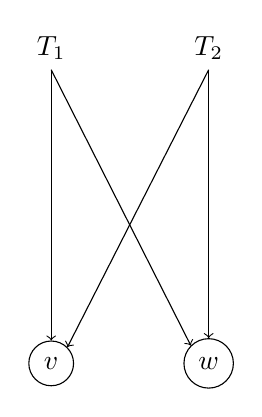
\begin{tikzpicture}
      \node (t1) at (-1,0) {$T_1$};
      \node (t2) at (1,0)  {$T_2$};
      \node (v) [draw,shape=circle] at (-1,-4) {$v$};
      \node (w) [draw,shape=circle] at (1,-4)  {$w$};

      \draw [->] (t1.south) -- (v.north);
      \draw [->] (t1.south) -- (w.north west);
      \draw [->] (t2.south) -- (v.north east);
      \draw [->] (t2.south) -- (w.north);
    \end{tikzpicture}
    \caption{Sequential Consistency}
  \end{subfigure}
  \begin{subfigure}{0.3\textwidth}
    \centering
    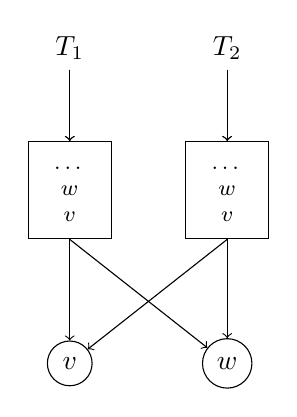
\begin{tikzpicture}
      \node (t1) at (-1,0) {$T_1$};
      \node (t2) at (1,0)  {$T_2$};
      \node (v) [draw,shape=circle] at (-1,-4) {$v$};
      \node (w) [draw,shape=circle] at (1,-4)  {$w$};

      \node (bt1) [draw] at (-1,-1.8) {\footnotesize\begin{tabular}{c} \ldots \\\midrule $w$ \\\midrule $v$ \end{tabular}};
      \node (bt2) [draw] at (1,-1.8) {\footnotesize\begin{tabular}{c} \ldots \\\midrule $w$ \\\midrule $v$ \end{tabular}};

      \draw [->] (t1) -- (bt1);
      \draw [->] (t1) -- (bt1);
      \draw [->] (t2) -- (bt2);
      \draw [->] (t2) -- (bt2);

      \draw [->] (bt1.south) -- (v);
      \draw [->] (bt1.south) -- (w);
      \draw [->] (bt2.south) -- (v);
      \draw [->] (bt2.south) -- (w);
    \end{tikzpicture}
    \caption{Total Store Order}
  \end{subfigure}
  \begin{subfigure}{0.3\textwidth}
    \centering
    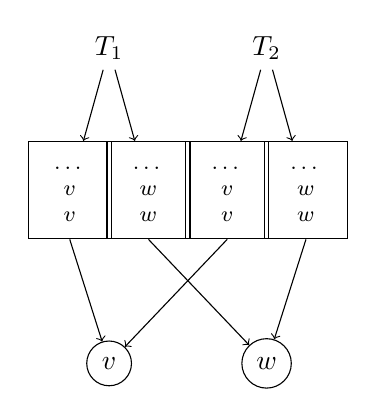
\begin{tikzpicture}
      \node (t1) at (-1,0) {$T_1$};
      \node (t2) at (1,0)  {$T_2$};
      \node (v) [draw,shape=circle] at (-1,-4) {$v$};
      \node (w) [draw,shape=circle] at (1,-4)  {$w$};

      \node (bt1v) [draw] at (-1.5,-1.8) {\footnotesize\begin{tabular}{c} \ldots \\\midrule $v$ \\\midrule $v$ \end{tabular}};
      \node (bt1w) [draw] at (-0.5,-1.8) {\footnotesize\begin{tabular}{c} \ldots \\\midrule $w$ \\\midrule $w$ \end{tabular}};
      \node (bt2v) [draw] at (0.5,-1.8) {\footnotesize\begin{tabular}{c} \ldots \\\midrule $v$ \\\midrule $v$ \end{tabular}};
      \node (bt2w) [draw] at (1.5,-1.8) {\footnotesize\begin{tabular}{c} \ldots \\\midrule $w$ \\\midrule $w$ \end{tabular}};

      \draw [->] (t1) -- (bt1v);
      \draw [->] (t1) -- (bt1w);
      \draw [->] (t2) -- (bt2v);
      \draw [->] (t2) -- (bt2w);

      \draw [->] (bt1v.south) -- (v);
      \draw [->] (bt1w.south) -- (w);
      \draw [->] (bt2v.south) -- (v);
      \draw [->] (bt2w.south) -- (w);
    \end{tikzpicture}
    \caption{Partial Store Order}
  \end{subfigure}
  \caption{Example of write buffering for two threads and two \texttt{CRef}s.}
  \label{fig:wb}
\end{figure}

We divide concurrency operations into three categories: \emph{synchronised}
operations impose a \emph{memory barrier}, which commits all buffered writes;
\emph{partially synchronised} operations commit one or more buffered writes to
the same \verb|CRef|; and \emph{unsynchronised} operations never cause a commit.

\paragraph{Phantom Threads}
In a sequentially consistent memory model, the set of runnable threads is
exactly the set of threads created by forking which are not blocked.  Under
relaxed memory, however, this is not the case.  For each write buffer, we
introduce one \emph{phantom thread}.  When scheduled, a phantom thread will
commit the oldest write in its corresponding buffer.

This may seem like an odd approach: why create new threads to model relaxed
memory?  The advantage is that systematic concurrency testing techniques assume
there is only one source of nondeterminism: the scheduler.  If a second source
is added, such as when writes are committed, it is difficult to integrate this
with existing algorithms.  By using phantom threads, the two sources of
nondeterminism are unified, and existing algorithms just work.  We take this
approach from \cite{zhang2015}.

\section{Testing Concurrent Programs}
\label{sec:dejafu-testing}

\dejafu{} uses a combination of dynamic partial-order reduction and
schedule bounding to test programs, by default.  Controlled random
scheduling using a fixed number of executions is also available.  To
make the tool easier to use, we provide a collection of different
testing functions, with varying levels of detail exposed, hoping that
the defaults will suffice for most users.  At one end of the scale we
have the \verb|autocheck| function, which looks for deadlocks,
uncaught exceptions in the main thread, and nondeterminism.  At the
other end of the scale is the \verb|dejafuDiscard| function which
exposes all the controls.

A \dejafu{} test has the following components:

\begin{itemize}
\item The testing algorithm to use plus any configuration it needs.
  The default is DPOR with schedule bounding.
\item A function to optionally discard results or traces as they are
  produced, and so not considering them when determining if the test
  passes.  This is a concession to performance: execution traces can
  take up a lot of memory, but typically we are only interested in a
  subset of them.
\item The memory model.  The default is total store order (TSO), as it
  is closest to the behaviour of an x86 processor\cite{owens2009},
  which is what the user probably has.
\item The \verb|MonadConc| action to test.
\item A named predicates, where a predicate is a function from the
  final list of results and traces to an indication of success or
  failure with an optional list of failing traces to display to the
  user.
\end{itemize}

\paragraph{Dependency Relation}
Correct DPOR relies on a dependency relation between pairs of actions
in a schedule trace.  This relation may be pessimistic, but cannot be
optimistic.  A pessimistic relation could claim that two actions are
related when they do not affect each other; an optimistic relation
could claim that two actions are unrelated when they do affect each
other.  A pessmistic relation may lead to exploring redundant
schedules, an optimistic relation may lead to missing distinct ones.

For ease of explanation, DPOR algorithms in the literature are
presented for small languages.  A paper will typically start with a
sentence like ``we assume a core concurrent language of reads and
writes to shared variables, and locks.''  The Haskell concurrency API
is richer than this, and the implicit dependencies between actions
(such as which actions impose a memory barrier) are not documented.
The dependency relation we now use in \dejafu{} was derived by running
small test cases many thousands of times.

We express our dependency relation in three parts: a relation on
\emph{thread actions}, which are entries in the trace; a relation on
\emph{thread action} and \emph{lookahead values}, which are forecasts
of what a thread will do, available to the scheduler; and a relation
on \emph{action types}, a simplification of thread actions.  Thread
actions contain more information than lookahead values, which contain
more information than action types.  We use this layered approach to
make use of this extra information to improve dependency detection
where possible.  \lstref{deprel-simp} shows a simplified view of our
relations.  \appref{deprel} shows the full dependency relation.

\begin{listing}
  \begin{minted}{haskell}
dependency :: ThreadId -> ThreadAction -> ThreadId -> ThreadAction -> Bool
dependency tid1 ta1 tid2 ta2
  | ...       = True
  | ...       = False
  | otherwise = dependency' tid1 ta1 tid2 (rewind ta2) &&
                dependency' tid2 ta2 tid1 (rewind ta1)

dependency' :: ThreadId -> ThreadAction -> ThreadId -> Lookahead -> Bool
dependency' tid1 ta tid2 lh
  | ...       = True
  | ...       = False
  | otherwise = dependentActions (simplifyAction    ta)
                                 (simplifyLookahead lh)

dependentActions :: ActionType -> ActionType -> Bool
dependentActions = ...
  \end{minted}
  \caption{A simplified view of the \dejafu{} dependency relations.}\label{lst:deprel-simp}
\end{listing}

For our dependency relation to be correct, we require some consistency
rules:

\begin{description}
\item[Commutativity (1)]
  $\mathrm{dependency}~x~y = \mathrm{dependency}~y~x$
\item[Commutativity (2)]
  $\mathrm{dependentActions}~x~y = \mathrm{dependentActions}~y~x$
\item[Consistency (1)]
  $\mathrm{dependency}~x~(t,y) \Rightarrow \mathrm{dependency'}~x~(t, \mathrm{rewind}~y)$
\item[Consistency (2)]
  $\mathrm{simplifyLookahead} = \mathrm{simplifyAction} \circ \mathrm{rewind}$
\end{description}

We establish these conditions through the syntactic structure of the
implementation.  Each function is a straightforward enumeration of
cases with attached side-conditions, which makes commutativity
apparent.  The more pessimistic \verb|dependency'| function is similar
to the more accurate \verb|dependency| function, but with less
information available, which makes consistency apparent.  We also
include these properties in the \dejafu{} testsuite to ensure they are
not inadvertently broken.

Recall that we divide thread actions into \emph{synchronised}, which
impose a memory barrier; \emph{unsynchronised}, which do not; and
\emph{partially synchronised}, which synchronise a single \verb|CRef|.
The \verb|dependentActions| function is defined in terms of this
synchronisation, and corresponds to the dependency relation for a core
concurrent language as would typically be used to introduce a new DPOR
algorithm.  The cases are:

\begin{enumerate}
\item Any two operations (excluding commits) on the same \verb|CRef|
  are dependent, other than two reads.
\item A write to a \verb|CRef| and a commit are \emph{not} dependent
  if the write buffer corresponding to the \verb|CRef| is not
  empty\cite{linden2013}.
\item A read of a \verb|CRef| is dependent with any action which
  imposes a memory barrier, if there are buffered writes.
\item A commit to a \verb|CRef| is dependent with any action which
  imposes a memory barrier.
\item Two actions involving the same \verb|CRef| where at least one
  would synchronise it are dependent.
\item Two actions involving the same \verb|MVar| are dependent.
\end{enumerate}

So, through the lens of \verb|dependentActions|, Haskell is a small
concurrent language with synchronised and unsynchronised shared
variables and memory barriers.  The other cases which are handled by
\verb|deprel| and \verb|deprel'| are: lifted \verb|IO| actions,
exceptions, STM transactions, and getting and setting the number of
capabilities.

\paragraph{Sleep Sets}
The sleep set optimisation is a complementary approach to
DPOR\cite{flanagan2005,godefroid1996} which we use to further reduce
schedules explored.  The intuition is as follows: if we have a choice
of two scheduling decisions, $t_{1}$ and $t_{2}$, after trying out
$t_{1}$ there is no point in making the sequence of decisions
$t_{2}t_{1}$ unless $t_{1} \dependent t_{2}$.  This is because all
states reachable from $t_{1}$ have already been explored, so the only
way a new state could arise is if $t_{1}$ had a different effect, and
that is what it means for two transitions to be dependent.

Formally, we augment each state $s$ with a \emph{sleep set}, these are
the transitions enabled in $s$ but which we will not make.  The
initial state has an empty sleep set.  Let $T$ be the transitions that
have been selected to be explored from $s$.  We proceed as follows:
take a transition $t_{1}$ out of $T$.  The sleep set associated with
the state reached after executing $t_{1}$ from $s$ is the sleep set
associated with $s$ with all transitions that are dependent with
$t_{1}$ removed.  Let $t_{2}$ be a second transition taken out of $T$.
The sleep set associated with the state reached after executing
$t_{2}$ from $s$ is the sleep set associated with $s$ augmented with
$t_{1}$, minus all transitions that are dependent with $t_{2}$.  We
continue until all transitions in $T$ have been explored, at each step
adding the previously taken transitions to the sleep set of the new
state, and removing the dependent transitions.

\paragraph{Schedule Bounding}
\dejafu{} supports pre-emption bounding\cite{musuvathi2007}, fair
bounding\cite{musuvathi2008}, and length bounding.  Fair and length
bounding allow the testing of cyclic or potentially infinite
state-spaces, at the cost of potentially confusing the user by
aborting the execution of their program when it is still runnable.
All three bounds are enabled by default, but can be selectively
disabled or customised.

\paragraph{Daemon Threads}
A daemon thread is a thread which is automatically killed after the
last non-daemon thread terminates.  They do not prevent termination of
the program.  In Haskell, every thread other than the main thread is a
daemon thread, so as soon as it terminates the whole program
terminates.  This is a problem for DPOR, as it makes the last action
of the execution dependent with everything else in the program!

Consider this small example program:

\begin{minted}{haskell}
main = do
  v <- newEmptyMVar
  fork (myThreadId >> putMVar v "hello world")
  tryReadMVar v
\end{minted}

There are two possible results: \verb|Nothing|, and
\verb|Just "hello world"|, we would like to see both of these.
However, there is no dependency between \verb|myThreadId| and
\verb|tryReadMVar|, so if the deterministic scheduler used favours the
main thread, we may not see the second execution.  Introducing a
dependency between the last action of the execution and everything
else solves this.  Now consider this example:

\begin{minted}{haskell}
main = do
  v <- newEmptyMVar
  fork (myThreadId >> myThreadId >> putMVar v "hello world")
  tryReadMVar v
\end{minted}

The forked thread now performs two calls to \verb|myThreadId|.  If the
\verb|tryReadMVar| happens after the second, we get the same result as
if it happened after the first.  Normally, DPOR would prevent this
redundancy, but by introducing a dependency between the final action
and everything else, we have told the algorithm that it is \emph{not}
redundant!  In general, introducing a dependency like this will lead
to many redundant executions which we would otherwise avoid.

The solution we adopt is to change the deterministic scheduler.  If
the scheduler has a choice of actions, where one or more will cause
the main thread to terminate, it makes its choice as usual, and then
records every other decision as a backtracking point.  By ensuring
that every other decision is tried at least once, we do not need to
introduce an additional dependency between the final action of the
main thread and everything else, and can just let DPOR do its job as
usual.

\section{Soundness and Completeness}
\label{sec:dejafu-correctness}

Correctness for \dejafu{} breaks down along a natural separation in
the theory: correctness of a single execution of a concurrent program,
and correctness of the testing framework around this which discovers
new executions.  We can state correctness as ``nothing is missed and
nothing is made up,'' or:

\begin{description}
\item[Soundness] \dejafu{} only reports results of the program which
  could arise under normal execution.
\item[Compleness] \dejafu{} reports all results of the program which
  could arise under normal execution, taking any schedule bounds into
  account.
\end{description}

There is also the concern of correctness of the implementation with
respect to the theory.  We do not concern ourselves with that issue in
this thesis, only noting that humans are fallible and that there have
been bugs in \dejafu{} before now.  There are almost certainly still
bugs.  Whenever a bug is discovered, a test reproducing it is added to
the testsuite and the underlying issue is fixed.

\subsection{Correct Execution}

Correctness of execution asks whether the result of an arbitrary
execution of \dejafu{}'s testing implementation can be obtained in
reality; and, furthermore, do all real-world executions correspond to
a possible execution under \dejafu{}?  Both of these come with the
caveat that the behaviour can be different, as long as this difference
can't be observed.

\paragraph{Program Behaviour}
There is no standard for concurrent Haskell, there is only what GHC
provides.  The behaviour of many operations is clear, but not so for
others.  \verb|CRef| operations are particularly complicated, as their
behaviour depends on the underlying memory model, which is
unspecified.  We chose TSO, but ignore the possibility that the GHC
optimiser or code generator could affect the memory model.

We justify the correctness of our implementation with comprehensive
testing: there are many test cases, checking that \dejafu{} exhibits
behaviours which we consider realistic.  The relaxed memory
implementation is particularly difficult to test, for that we have a
collection of \emph{litmus tests} which we can evaluate many thousands
of times using \verb|IO| and compare to the results \dejafu{}
produces.

Furthermore, there are some intentional semantic differences for
practical concerns.  For example, GHC can sometimes detect deadlocks
involving only a subset of the threads, and throw an exception to the
threads signalling this.  We cannot do this.

So the behaviour of \dejafu{} is not correct, but we hope it is as
close as can reasonably be achieved.

\paragraph{Possible Executions}
Our stepwise execution of concurrent programs allows a scheduling
decision to be made between each primitive action, which doesn't
correspond to how GHC handles scheduling:

\begin{bquote}{Control.Concurrent module documentation\footnote{\url{https://hackage.haskell.org/package/base-4.10.0.0/docs/Control-Concurrent.html\#g:13}}}
  GHC implements pre-emptive multitasking: the execution of threads
  are interleaved in a random fashion.  More specifically, a thread may
  be pre-empted whenever it allocates some memory, which unfortunately
  means that tight loops which do no allocation tend to lock out other
  threads (this only seems to happen with pathological benchmark-style
  code, however).
\end{bquote}

So there are executions involving the pre-emption of the evaluation of
non-terminating expressions which are possible under GHC but not under
\dejafu{}.  Whether this can be used to produce different outputs is
unclear.

\subsection{Correct Testing}

Correctness of testing asks whether the schedule prefixes generated by
the DPOR machinery are valid; and, furthermore, are there any possible
results for which no schedule will be generated?  This is different to
the testing framework generating every schedule, as that is precisely
what DPOR tries to avoid.

\paragraph{Prefix Validity}
Executions are stored internally as a stack, shown in \lstref{dpor}.
The sequence of thread IDs corresponding to this stack represents a
complete execution of the program.  There is a unique initial state,
where only the initial thread is runnable and nothing has been done.

\begin{listing}
  \begin{minted}{haskell}
data DPOR = DPOR
  { dporRunnable :: Set ThreadId
  -- ^ What threads are runnable at this step.
  , dporTodo     :: Map ThreadId Bool
  -- ^ Follow-on decisions still to make, and whether that decision
  -- was added conservatively due to the bound.
  , dporNext     :: Maybe (ThreadId, DPOR)
  -- ^ The next decision made. Executions are explored in a
  -- depth-first fashion, so this changes as old subtrees are
  -- exhausted and new ones explored.
  , dporDone     :: Set ThreadId
  -- ^ All transitions which have been taken from this point,
  -- including conservatively-added ones.
  , dporSleep    :: Map ThreadId ThreadAction
  -- ^ Transitions to ignore (in this node and children) until a
  -- dependent transition happens.
  , dporTaken    :: Map ThreadId ThreadAction
  -- ^ Transitions which have been taken, excluding
  -- conservatively-added ones. This is used in implementing sleep
  -- sets.
  } deriving (Eq, Show)
  \end{minted}
  \caption[The \dejafu{} DPOR state.]{The DPOR state is a stack of scheduling decisions.}\label{lst:dpor}
\end{listing}

There are some basic well-formedness properties associated with a
\verb|DPOR| value: every thread in the to-do set is runnable; every
thread in the done set is runnable; the done and to-do sets are
disjoint; no thread in the sleep set is also in the done set; the
taken set is the done set excluding the sleep set; the next-taken
decision (if there is one) is in the runnable set and not in the to-do
or sleep sets; and these properties hold recursively.

A generated schedule prefix is one of the longest sequence of taken
decisions followed by a single to-do decision possible.  This
corresponds to a depth-first search of the space of schedules.  As
long as the well-formedness properties hold, and the runnable sets are
correctly recorded during execution, then a generated schedule prefix
will be valid.

\paragraph{Schedule Completeness}
The simplest notion of completeness of interest here is that for all
results possible by executing a given program, the DPOR machinery can
give that result.  However, as schedule bounding is involved, this is
not the case.  So we have two slightly different notions of
completeness:

\begin{enumerate}
\item When all schedule bounds are disabled, all possible results show
  up under testing.
\item For all sets of bounds, all results possible subject to those
  bounds show up under testing with the same bounds.
\end{enumerate}

Property (2) implies property (1).  We use \cite{coons2013} as our
core DPOR algorithm, which establishes property (2).

\section{Case Studies}
\label{sec:dejafu-casestudies}

\blindtext

\subsection{The auto-update Package}
\subsection{Search Party}
\subsection{The Par Monad}

\section{\dejafu{} in the Wild}
\label{sec:dejafu-evaluation}

\blindtext

\subsection{Richness of the Abstraction}
\subsection{Porting Code}
\subsection{Integration with Existing Tools}

\section{Conclusions and Future Work}
\label{sec:dejafu-conclusions}

\blindtext
